\chapter{Experimental Evaluation}
\label{chap:experimental-evaluation}
	\todo{Add something about the web interface (screenshots, etc.)}
	
	In this chapter we evaluate our implementation of the system for transforming data in the relational model to the document model and vice versa described in \cref{chap:tale-of-two-data-models}.  We cover the implementation details in \cref{sec:implementation}, and the methodology and evaluation in \cref{sec:runtime-evaluation}.
	
	\section{Implementation}
	\label{sec:implementation}
		The system was implemented in Clojure, which \textcquote{clj-home}{is a dynamic programming language that targets the \gls{jvm}}.  Clojure was chosen due to its rich, immutable, and persistent data structures, excellent concurrency support, and seamless \gls{jvm} interoperability.  These features were discussed in detail in \cref{sec:features-of-clojure}.
		
		\subsection{Code Base Statistics}
			The system consists of over 800 lines of Clojure, along with approximately 550 lines of Python.  The Python code is used to construct the data set by crawling the course information site, as well as to aggregate the benchmark data produced by the system, producing graphs.
			
			All development has occurred on GitHub \cite{molly-repo}.  The use of Git and GitHub permits collaboration between researchers.  With the code publicly available, future researchers may study and run it.
	
	\section{The Data Corpus}
	\label{sec:data-corpus}
		The data corpus was derived from the \gls{uoit} mycampus database.  An \gls{html} crawler was written in Python that scraped the information from the \gls{uoit} class schedule search page.  This data was parsed, normalized, then placed in a SQLite database.
		
		The data corpus consists of numerous classes of objects.  These are:  courses (\cref{tbl:corpus-course}), instructors (\cref{tbl:corpus-instructor}), schedules (\cref{tbl:corpus-schedule}), sections (\cref{tbl:corpus-section}), and teaches (\cref{tbl:corpus-teach}).  A graph representation of how these classes of objects are related can be found in \cref{fig:schema-graph}.  The data corpus is defined in \cref{chap:data-corpus-def}
		
		The number of objects, as of the publication of this thesis, can be found in \cref{tbl:data-corpus-count}.
		
		\begin{table}[H]
			\centering
			\begin{tabular}{lr}
			\toprule
			Class & Count \\
			\midrule
			Course & 1340 \\
			Instructor & 849 \\
			Schedule & 25755 \\
			Section & 14463 \\
			Teaches & 15358 \\
			\bottomrule
			\end{tabular}
			
			\caption{Number of objects in data corpus, grouped by class}
			\label{tbl:data-corpus-count}
		\end{table}
	
	\section{Runtime Evaluation}
	\label{sec:runtime-evaluation}
		Scripts were written to coordinate the execution, collection, and transformation of the performance data of our implementation.
		
		\subsection{Methodology}
			We used Criterium\footnote{\url{http://hugoduncan.org/criterium/}} to handle the execution of the benchmarks as it handles unique concerns stemming from benchmarking on the \gls{jvm}.  These issues, identified by \citeauthor{rob-java-bench-08} \cite{rob-java-bench-08}, include:
			
			\begin{itemize}
				\item Statistical processing of multiple evaluations
				\item Inclusion of a warm-up period, designed to allow the JIT compiler to optimize its code
				\item Purging of the garbage collector before testing, to isolate timings from GC state prior to testing
				\item A final forced garbage collection after testing to estimate impact of cleanup on the timing results
			\end{itemize}
		
			This requires a much longer runtime as each function must be invoked numerous times.
			
			During evaluation, Criterium collects performance metrics.  Upon completion of the evaluation, it performs statistical analysis of these metrics using the bootstrap procedure developed by \citeauthor{efron-87} \cite{efron-87}.  These metrics include mean, samples, variance, quartiles, outliers, and more.
		
			\subsubsection{Data Collection}
			\label{sec:data-collection}
				The performance metrics computed by Criterium are returned as a Clojure map data structure.  The evaluation process may take several hours to complete, necessitating a separation between data collection and post-processing.  These metrics are stored offline for further processing.
				
				In order to utilize the Clojure output in Python, a data interchange format (\gls{json}) is used.  The benchmark function writes the Criterium performance analysis out as a \gls{json} string to stdout and the output is captured by the benchmark script.  An example of this \gls{json} output is given in \cref{fig:criterium-json-output}.
				
				\begin{figure}[H]
					\centering % Pointless, but who knows in the future.
					\begin{verbatim}
                    [{
                        "max-hops": ...,
                        "method": ...,
                        "results": {
                            "execution-count": ...,
                            "final-gc-time": ...,
                            "lower-q": [...],
                            "mean": [...],
                        ...
                    }, ...]
					\end{verbatim}
					
					\caption{Partial \gls{json} output from Criterium.}
					\label{fig:criterium-json-output}
				\end{figure}
		
		\subsection{Performance}
		\label{sec:performance}
			Performance was measured for the various system components.  An analysis of the metrics collected is presented in this section.
			
			\subsubsection{Indexing}
				The indexing process is computationally intensive but short lived.  After the initial \gls{jvm} warmup period, the time required to construct the index scales with the number of named tuples and relations between them.
				
				\begin{table}[H]
					\centering
					\begin{tabular}{ll}
						\toprule
						Number of Groups & Elapsed Time (s) \\
						\midrule
						0 & 11.800 \\
						1 & 12.446 \\
						2 & 19.771 \\
						\bottomrule
					\end{tabular}
					
					\caption{Indexing time growth by number of entity groups, averaged over 5 runs}
					\label{tbl:index-growth-entity-groups}
				\end{table}
				
				We see in \cref{tbl:index-growth-entity-groups} the indexing time increases minimally between 0 and 1 group.  The number of entity groups added by the first entity schema is relatively small.  Contrast this to the indexing time between 1 and 2 groups, which increases considerably.  The number of entity groups also grew considerably, explaining the time increase.
			
			\subsubsection{Graph Search}
				The worst-case performance of \gls{bfs} is \(\mathcal{O}(n^2)\).  This is reflected in \cref{fig:method-runtime-tkes-25} which follows an exponential growth curve.  In an attempt to mitigate the rapid increase in search time, concurrent variants of \gls{bfs} were also implemented and benchmarked.
				
				\begin{figure}[H]
					\centering
					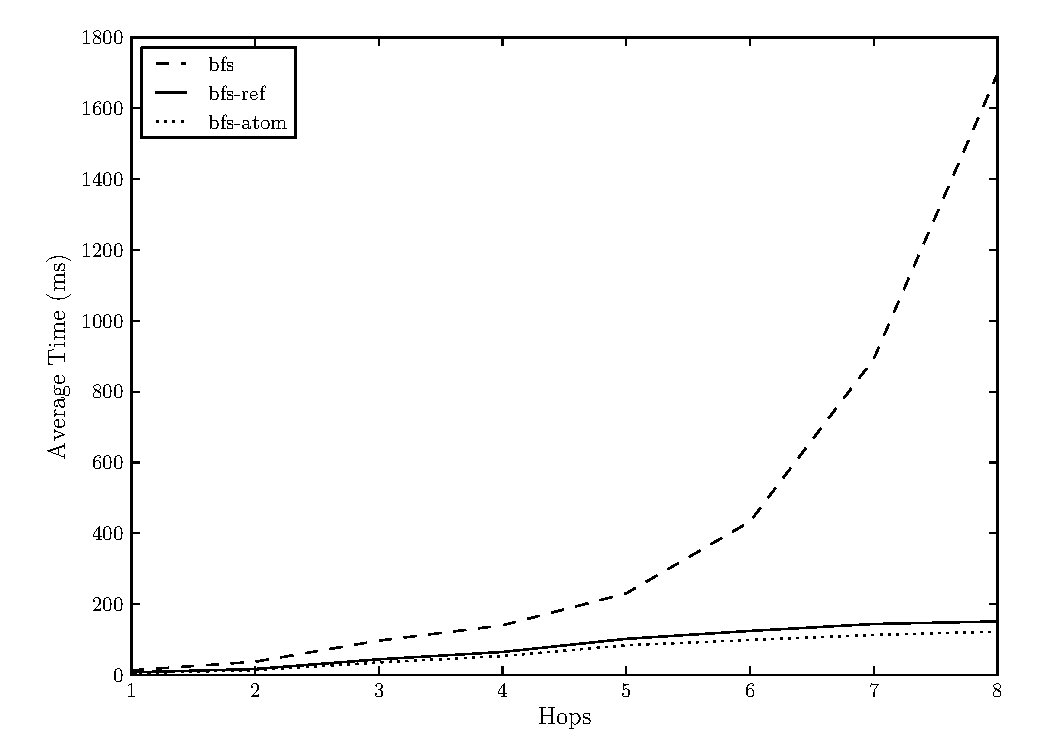
\includegraphics[scale=0.9]{figures/charts/growth.pdf}
					\caption{Growth of each graph search algorithm implementation by number of hops}
					\label{fig:growth}
				\end{figure}
				
				We see in \cref{fig:growth} the rate of growth of \gls{bfs} is as expected.  The rate of growth of \gls{bfs} with references and \gls{bfs} with atoms is nearly linear.  The atom implementation is slightly more performant as it lacks some of the overhead associated with references.
				
				\begin{figure}[H]
					\begin{subfigure}[b]{.5\linewidth}
						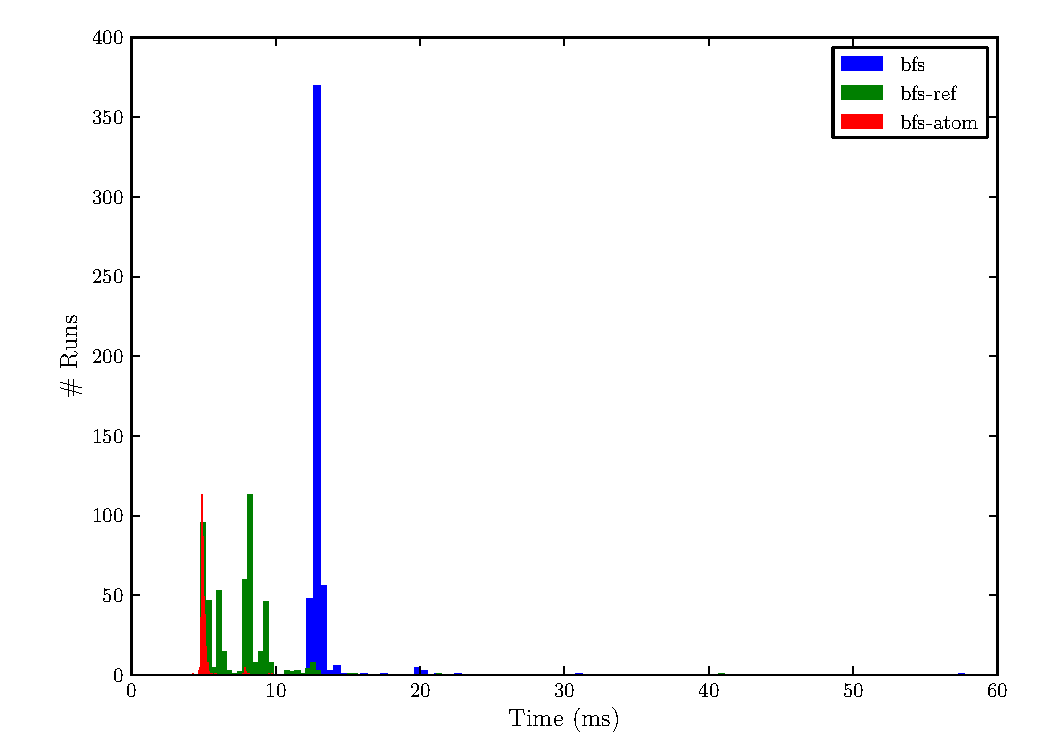
\includegraphics[scale=0.45]{figures/charts/1_hops.pdf}
						\caption{1 Hop}
						\label{subfig:1-hop}
					\end{subfigure}
					\begin{subfigure}[b]{.5\linewidth}
						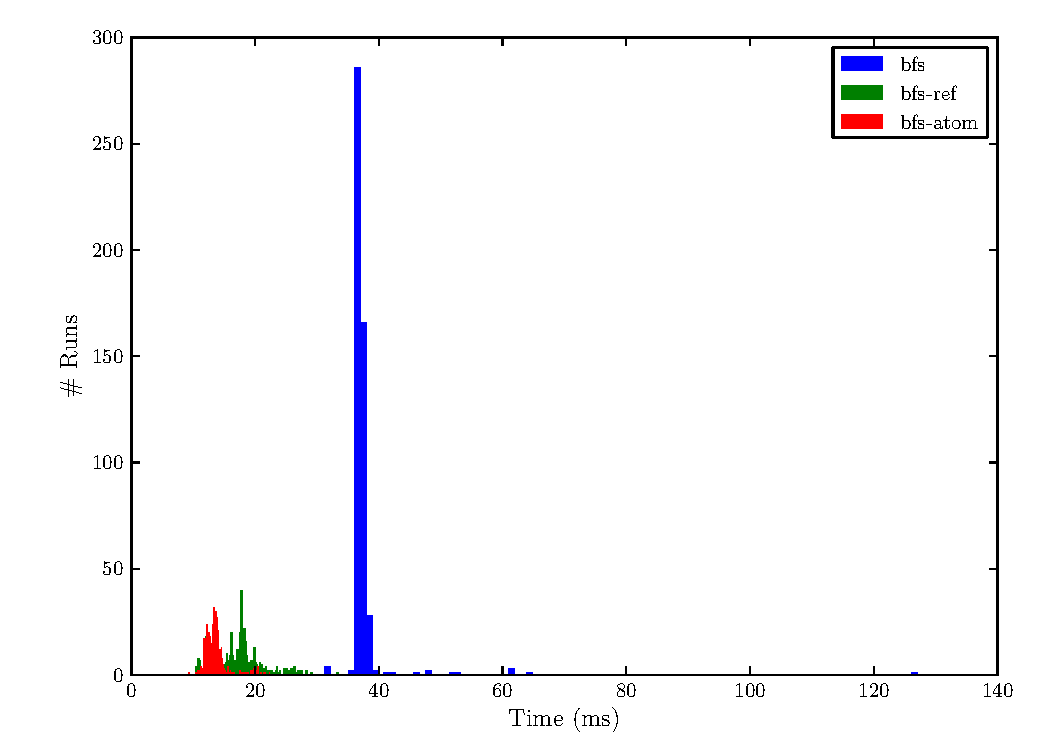
\includegraphics[scale=0.45]{figures/charts/2_hops.pdf}
						\caption{2 Hops}
						\label{subfig:2-hops}
					\end{subfigure}
				\end{figure}
				\begin{figure}[H]
					\ContinuedFloat
					\begin{subfigure}[b]{.5\linewidth}
						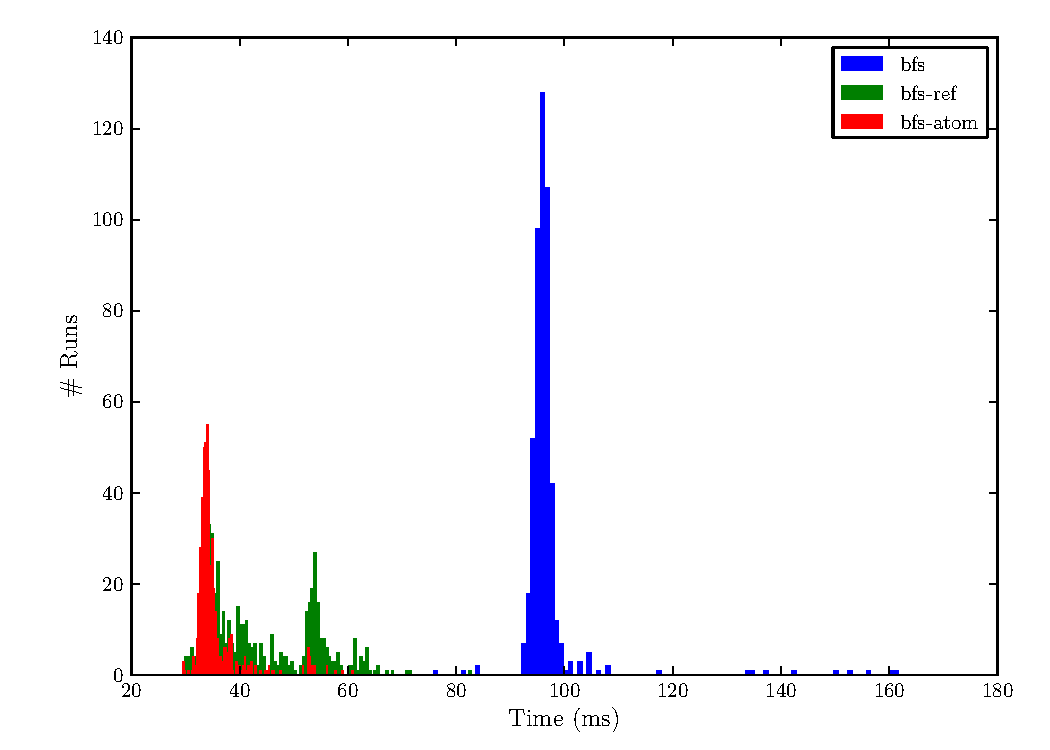
\includegraphics[scale=0.45]{figures/charts/3_hops.pdf}
						\caption{3 Hops}
						\label{subfig:3-hops}
					\end{subfigure}
					\begin{subfigure}[b]{.5\linewidth}
						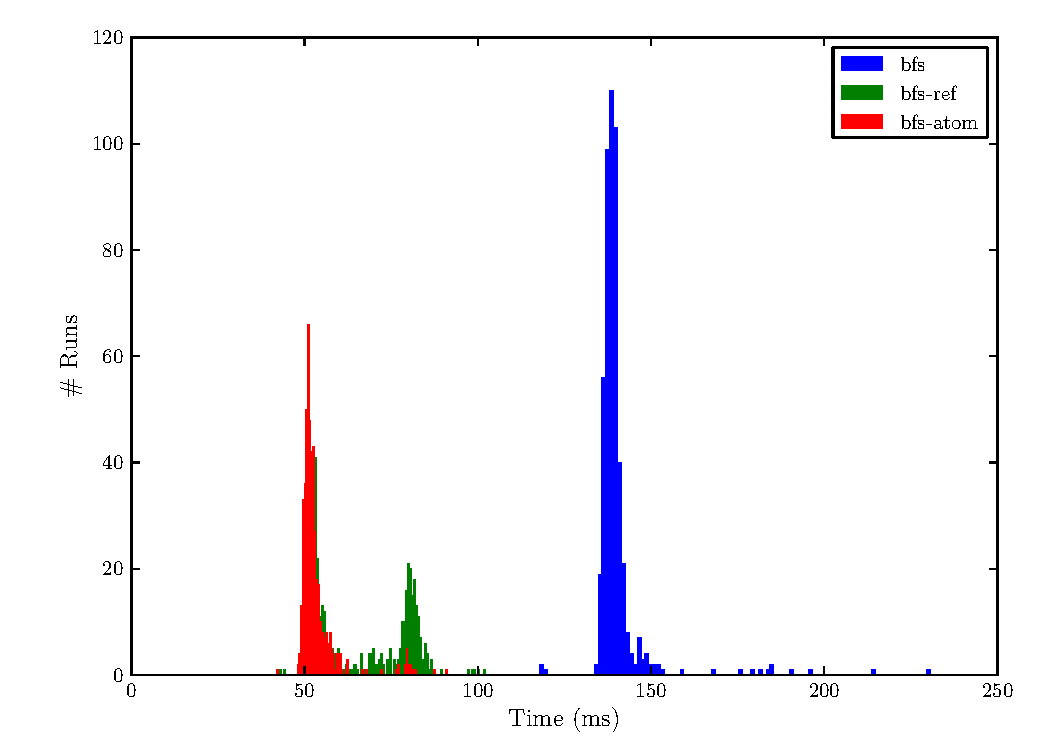
\includegraphics[scale=0.45]{figures/charts/4_hops.pdf}
						\caption{4 Hops}
						\label{subfig:4-hops}
					\end{subfigure}
				\end{figure}
				
				\begin{figure}[H]
					\ContinuedFloat
					\begin{subfigure}[b]{.5\linewidth}
						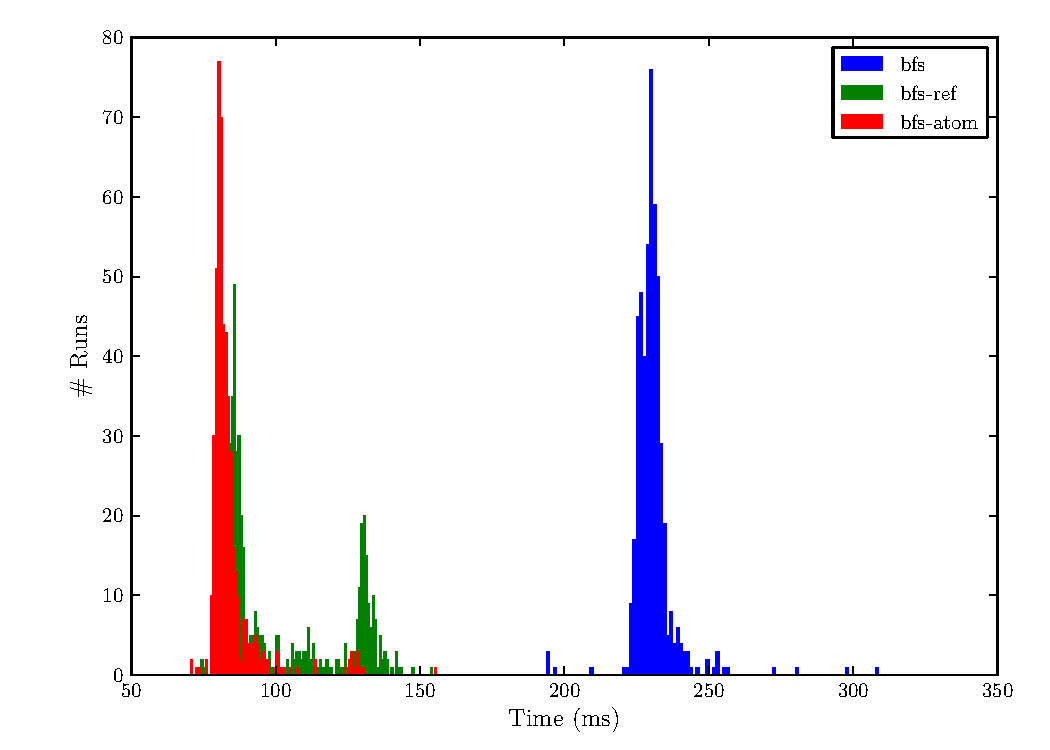
\includegraphics[scale=0.45]{figures/charts/5_hops.pdf}
						\caption{5 Hops}
						\label{subfig:5-hops}
					\end{subfigure}
					\begin{subfigure}[b]{.5\linewidth}
						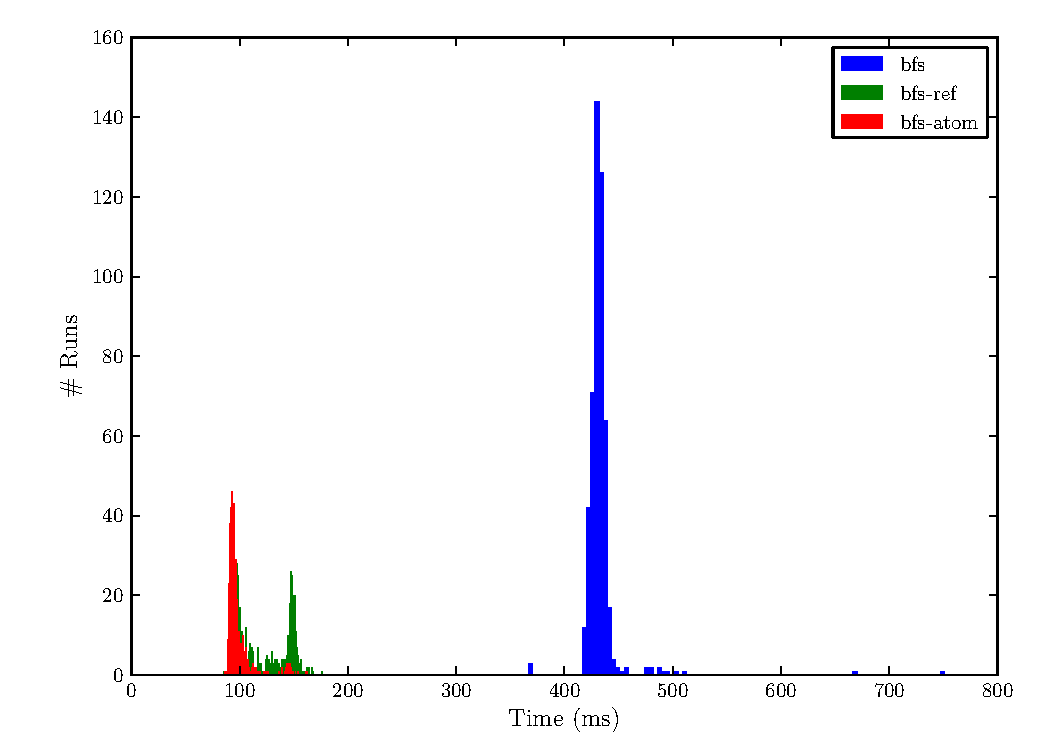
\includegraphics[scale=0.45]{figures/charts/6_hops.pdf}
						\caption{6 Hops}
						\label{subfig:6-hops}
					\end{subfigure}
				\end{figure}
				\begin{figure}[H]
					\ContinuedFloat
					\begin{subfigure}[b]{.5\linewidth}
						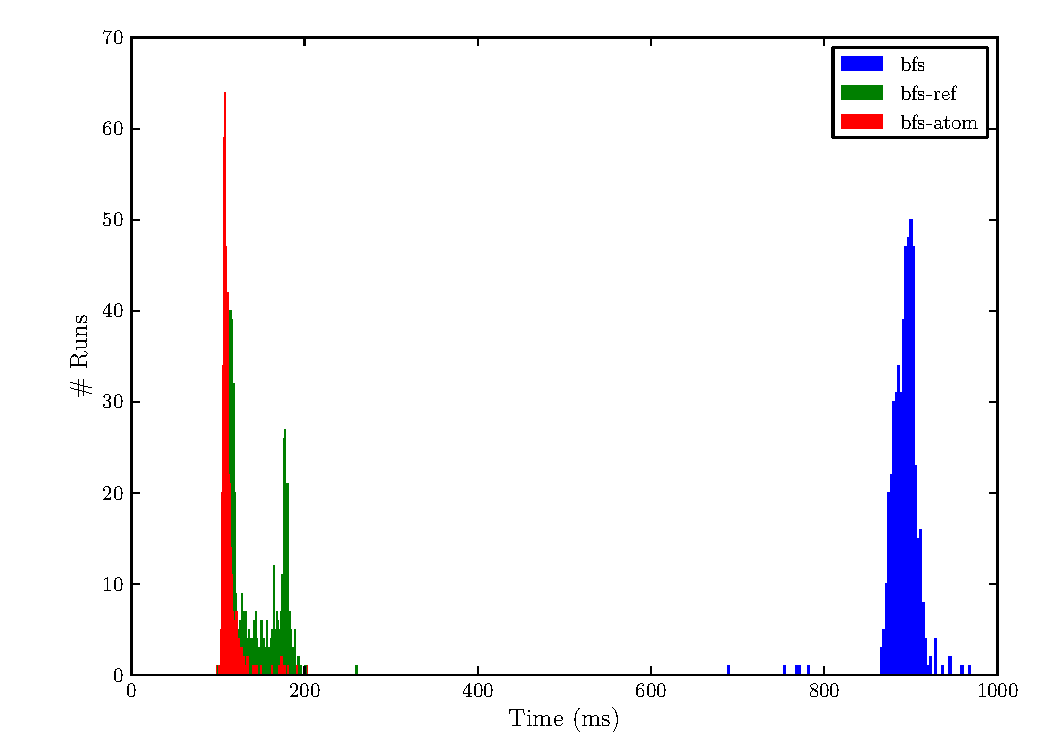
\includegraphics[scale=0.45]{figures/charts/7_hops.pdf}
						\caption{7 Hops}
						\label{subfig:7-hops}
					\end{subfigure}
					\begin{subfigure}[b]{.5\linewidth}
						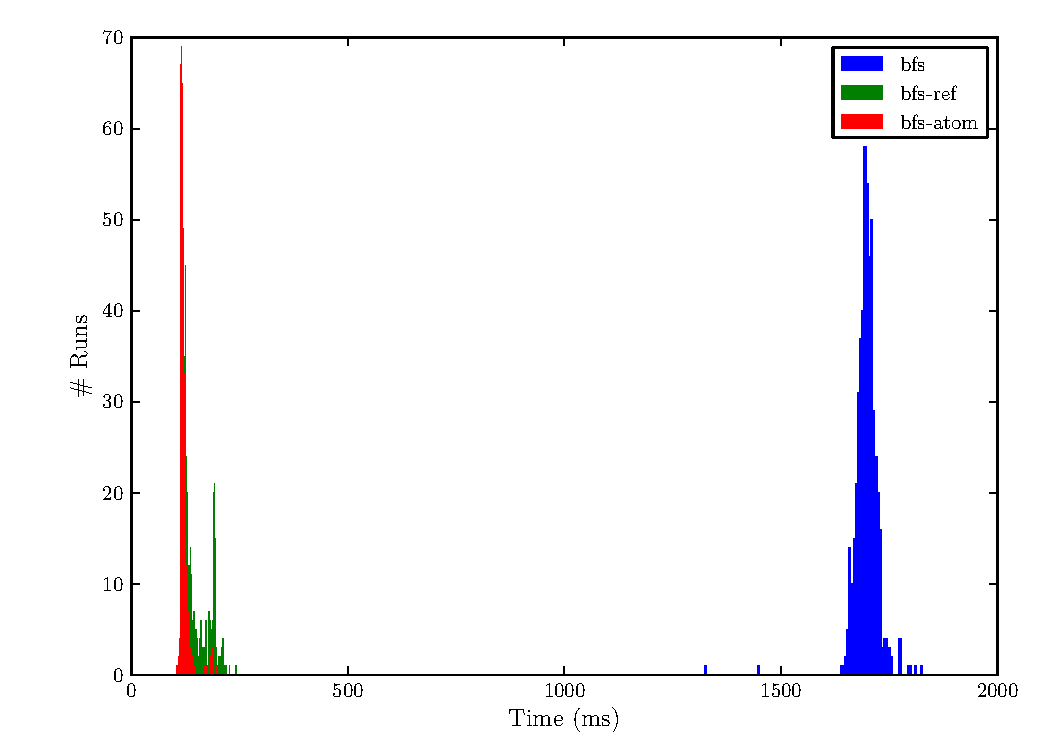
\includegraphics[scale=0.45]{figures/charts/8_hops.pdf}
						\caption{8 Hops}
						\label{subfig:8-hops}
					\end{subfigure}
					
					\caption{Distribution of samples per method, broken down by hops}
					\label{fig:distribution-hops}
				\end{figure}
				
				\todo{All captions must be at least 10pt}
				
				The difference in rate of growth is further illustrated in \cref{fig:distribution-hops}.  As seen previously, \cref{subfig:1-hop} shows little difference in runtime between the three methods.  The difference becomes clearer in \cref{subfig:2-hops}, and by \cref{subfig:8-hops}, the difference is obvious.
			
	\section{Conclusion}
	\label{sec:eval-conclusion}
		In evaluating the system, we came to several conclusions.
		
		Benchmarking any code is difficult.  The process may not have exclusive control over the processor, memory is paged in and out, disk I/O is cached, etc.  The \gls{jvm} complicates matters with \gls{jit} compilation and garbage collection.
		
		The growth of \gls{bfs} can be mitigated by the use of concurrency.  Clojure facilitated a natural transition from a classical implementation of \gls{bfs} to a highly concurrent one.